
\chapter{Finite Element spaces}\label{sec:fem}

In the previous lectures we have studied the properties of coercive problems in an abstract setting and described Ritz and Galerkin methods for the approximation of the solution to a PDE, respectively in the case of symmetric and non-symmetric bilinear forms.

\medskip
The abstract setting reads:
\begin{equation*}
\left\lvert
\begin{array}{l}
\mbox{Find $\uh\in\xVh\subset \xH$ such that:}\\[2ex]
a(\uh,\vh) = L(\vh)\quad,\;\forany  \vh \in \xVh
\end{array}
\right.
\end{equation*}
such that:
\begin{itemize}
\item $\xVh$ is a finite dimensional approximation space characterized by a discretization parameter $h$,
\item $a(\xDot,\xDot)$ is a continuous bilinear form on $\xVh\times\xVh$, coercive \wrt $\norm{\xDot}_{\xV}$,
\item $L(\xDot)$ is a continuous linear form.
\end{itemize}

Under these assumptions existence and uniqueness of a solution to the approximate problem holds owing to the Lax--Milgram Theorem and $\uh$ is called \textit{discrete solution}.
Provided this abstract framework which allows us to seek approximate solutions to PDEs, we need now to define the discrete space $\xVh$ and construct a basis $(\varphi_1,\cdots,\varphi_{\NxVh})$ of $\xVh$, $\NxVh = \dim(\xVh)$, on which the discrete solution is decomposed as
\begin{equation*}
\uh = \sum_{j=1}^{\NxVh} u_j\; \varphi_j
\end{equation*}
with $\lbrace u_j \rbrace$ a family of $\NxVh$ real numbers called \textit{global degrees of freedom} and $\lbrace \varphi_j \rbrace$ a family of $\NxVh$ elements of $\xVh$ called \textit{global shape functions}.

\medskip
Previously no assumption was made on the finite dimensional space $\xV_n$ aside from that $\xV_n \subset \xV$.
The change of notation to $\xV_h$ is to reflect that the discrete space $\xV_h$ will be caracterized more carefully as an \textit{approximation space} by constructing the shape functions and by defining the degrees of freedom.

\medskip
To construct the Finite Element space $\xVh$, three ingredients are introduced:
\begin{enumerate}
\item An admissible mesh $\meshT$ generated by a tesselation of domain $\dom$.
\item A reference Finite Element $\RefFE$ to construct a basis of $\xVh$ and define the meaning of $u_j$.
\item A mapping that generates a Finite Element $\FE$ for any cell in the mesh from the reference element $\RefFE$.
\end{enumerate}

\medskip
As a preliminary step the approximation of the Poisson problem in one dimension by linear Lagrange Finite Elements is described to give an overview of the methodology without hitting the technnical difficulties.
Concepts and notations for the discretization of the physical domain are then introduced.
Provided that all the requirements are identified, a framework for all the Finite Element methods is introduced by stating the definition of a Finite Element.
Finally, the generation of the Finite Element space from a reference Finite Element will be described.
Some examples of Finite Element spaces are listed at the end of the chapter.

%-------------------------------------------------------------------------------
\section{A preliminary example in one dimension of space}\label{sec:poisson_lagrange_p1}

For the sake of completeness, steps performed to derive a Galerkin method for the Poisson Problem \ref{pb:poisson} on $\dom = (0, 1)$ are sketched below to recapitulate the methodology.

\subsection{Weak formulation}

A solution is sought in the distributional sense by testing the equation against smooth functions,
\begin{equation*}
- \intD u''(x) v(x) \md x = \intD f(x) v(x) \md x\:,\qquad\forany v \in \xCinfc(\dom)
\end{equation*}
then reporting derivatives on the test functions using the integration by part
\begin{equation*}
- \intD u''(x) v(x) \md x = - \underbrace{[u'(x)v(x)]_0^1}_{= 0} + \intD u'(x) v'(x) \md x
\end{equation*}
the weak formulation consists of finding $u\in\xV$ such that
\begin{equation*}
\intD u'(x) v'(x) \md x = \intD f(x) v(x) \md x\:,\qquad\forany v \in \xV
\end{equation*}
given $f \in \xLtwo(\dom)$.
The choice of solution space and test space is guided by the equation and the data: in this case $\xV = \xHonec(\dom)$ since $v$ and $v'$ should be controlled in $\xLtwo(\dom)$, and homogeneous Dirichlet boundary conditions are imposed.

\subsection{Galerkin method}

The approximate problem by a Galerkin method consists of seeking a discrete solution $\uh$ in a finite dimensional space $\xVh \in \xV$, such that
\begin{equation*}
\intD \uh'(x) v'(x) \md x = \intD f(x) v(x) \md x\:,\qquad\forany v \in \xVh
\end{equation*}
and given a basis $\Fam{\varphi_j}$ of $\xVh$ any function $w\in\xVh$ can be written as
\begin{equation*}
w_h = \sum_{j=1}^{\NxVh} \underbrace{w_j}_{\in\,\xR}\;\varphi_j
\end{equation*}
with $\NxVh = \dim{\xVh}$, and moreover
\begin{equation*}
w'_h = \sum_{j=1}^{\NxVh} \underbrace{w_j}_{\in\,\xR}\;\varphi'_j
\end{equation*}
by simple application of the derivation on the linear combination.
Bounds of the sum will be omitted to simplify the notation,
\begin{equation*}
\sum_{j=1}^{\NxVh} \sim \sum_{j}
\end{equation*}
 when there is no possible confusion.

\medskip
Inserting the Galerkin decomposition in the weak formulation and using the commutativity of the derivation with the linear combinations,
\begin{equation*}
\intD \Bigl(\sum_{j} u_j\;\varphi'_j(x)\Bigr) \Bigl(\sum_{i} v_i\;\varphi'_i(x)\Bigr) \md x = \intD f(x) \Bigl(\sum_{i} v_i\;\varphi_i(x)\Bigr) \md x
\end{equation*}
and the integration can also commute with the linear combinations,
\begin{equation*}
\sum_{j} \sum_{i} u_j v_i \intD \varphi'_j(x)\varphi'_i(x) \md x = \sum_{i} v_i\intD f(x) \varphi_i(x) \md x
\end{equation*}
so that up to some cosmetic reordering, for any $v \in \xV$
\begin{equation*}
\sum_{i}  \sum_{j} v_i \intD \varphi'_i(x)\varphi'_j(x) \md x u_j = \sum_{i} v_i\intD f(x) \varphi_i(x) \md x
\end{equation*}
the relation to the linear system of algebraic equations becomes evident,
\begin{equation*}
\vecv^\trans \matA\;\vecu = \vecv^\trans \vecb
\end{equation*}
for any $\vecv = [v_i]\in \xR^\NxVh$, with
\begin{equation*}
\matA = \left[\intD \varphi'_j(x)\varphi'_i(x) \md x\right]_{ij},\quad\vecb = \left[\intD f(x) \varphi_i(x) \md x\right]_{i}
\end{equation*}
and the discrete solution is represented by the solution vector $\vecu = [u_j]\in \xR^\NxVh$.
Computing contributions $\matA_{ij}$ and $\vecb_i$ is possible as soon as the basis $\Fam{\varphi}_j$ is constructed explicitly.

\medskip
\begin{rmrk}
The choice of indices $i$ and $j$ in the previous expressions follows the usual convention for row and column indices. The matrix $\matA$ represents a linear application from the solution space $\xH$ to the trial space $\xV$: therefore the solution space is the column space, while the trial space is the row space.
In the case of Galerkin approximations where $\xH = \xV$ -- and even more when the bilinear form is symmetric -- it is tempting to choose the indices arbitrarily, but for the sake of consistency following the convention is recommended.
\end{rmrk}

\subsection{Construction of the discrete space}

A discretization of the computational domain $\bar\dom = [0,1]$ is constructed by partitioning the interval into disjoints subintervals $K_i = [x_{i}, x_{i+1}]$, $1\leq i \leq N_K$.
\begin{equation*}
\bar\dom = \displaystyle\Union_{i = 1}^{N_K} K_i\;,\qquad \Interior{K_i}\cap \Interior{K_j} = \Empty
\end{equation*}
The family of cells $\Fam{K_i}$ defines a \textit{mesh} noted $\meshT$.
A partition of $[0,1]$ into $N_K$ subintervals $[x_i, x_{i+1}]$ corresponds to a familiy of $N_K+1$ points $\Fam{x_i}$ which are the \textit{vertices} of the mesh $\meshT$.

\medskip
In this example the approximation space is constructed with piecewise linear Lagrange polynomials.
The chosen discrete space is
\begin{equation}\label{sp:lagrangeP1}
\xVh = \lbrace v \in \xC^0(\bar\dom)\cap\xHonec(\dom) : \forany K \in \meshT, v\rvert_{K} \in \xPone(K) \rbrace
\end{equation}
which consists of functions continuous over $\bar\dom$ that are linear on each cell $K$, and $\xVh \subset \xV$ so that the approximation is $\xHonec$--conformal.
A continuous piecewise linear function $v_h \in \xVh$ is the linear interpolate of $v\in\xV$ on $\meshT$ if $v_h = \Iop{\xVh}$ with the interpolation operator
\begin{equation}\label{fem:lagrange_interpolator}
\begin{array}{lclcl}
\Iop{\xVh} &:& \xV &\rightarrow& \xVh\\[2ex]
           & & v   &\mapsto    & \displaystyle\sum_{i=1}^{\NxVh} v(\xi_i) \varphi_i
\end{array}
\end{equation}
such that $\NxVh = \dim{\xVh}$ and $\Fam{\xi_i}$ is a family of $\NxVh$ distinct nodes.
In this particular case of a linear interpolation $\NxVh = N_K + 1$ and the family $\Fam{\xi_i}$ is identified with the vertices $\Fam{x_i}$.

\begin{figure}[h!]
\centering
\begin{tikzpicture}
  \begin{axis}[
    xmin=0.,
    xmax=1.,
    ymin=0.,
    ymax=1.1,
    axis x line*=bottom,
    axis y line*=center,
    /pgfplots/xtick={0., 0.2, ..., 1},
    /pgfplots/ytick={0., 0.2, ..., 1},
    width=\textwidth,
    height=\axisdefaultheight
    ]
    \addplot[darkblue, thick, domain=0:1, samples=100]{0.80*(sin(x*180.) - 0.4*sin(2.*x*180.))} node[right] at (75, 90) {$v\in\xV$};
    \addplot[black, domain=0:1, samples=6]{0.80*(sin(x*180.) - 0.4*sin(2.*x*180.))} node[left] at (35, 50) {$\Iop{\xVh} v\in\xVh$};
    \addplot[ybar, bar width=0pt, black, dotted, thin, domain=0:1, samples=6]{0.80*(sin(x*180.) - 0.4*sin(2.*x*180.))};
  \end{axis}
\end{tikzpicture}
\caption{The function $v(x) = 0.8 \sin(2\pi x) - 0.32 \sin(4\pi x)$ and its linear interpolate $\Iop{\xVh} v$ with $6$ equidistributed nodes.}
\end{figure}

\medskip
The construction of the basis $\lbrace\varphi_j\rbrace$ of $\xVh$ should produce a linear system that can be solved easily so the matrix should be as sparse as possible.
Given the expression of the contributions $\matA_{ij}$ the requirement is that functions $\varphi_j$ overlap as little as possible with each other: the support of $\varphi_j$ should be reduced so that contributions are non-zero only for neighbouring $\varphi_i$ functions; this choice is consistent with the locality of differential operators.

\begin{figure}[h!]
\centering
\begin{tikzpicture}
  \begin{axis}[
    xmin=0.,
    xmax=1.,
    ymin=0.,
    ymax=1.1,
    axis x line*=bottom,
    axis y line*=center,
    xtick={0.0,0.3,0.4,0.5,0.6,0.7,1.0},
    xticklabels={$0$, $x_{i-2}$, $x_{i-1}$, $x_{i}$, $x_{i+1}$, $x_{i+2}$, $1$},
    /pgfplots/ytick={0., 1.},
    width=\textwidth,
    height=\axisdefaultheight
    ]
    \addplot[black, dashed, domain=0.3:0.4]{10*(x-0.3)} node[above] {$\varphi_{i-1}$};
    \addplot[black, dashed, domain=0.4:0.5]{10*(0.5-x)};
    \addplot[black, domain=0.4:0.5]{10*(x-0.4)} node[above] {$\varphi_i$};
    \addplot[black, domain=0.5:0.6]{10*(0.6-x)};
    \addplot[black, dashed, domain=0.5:0.6]{10*(x-0.5)} node[above] {$\varphi_{i+1}$};
    \addplot[black, dashed, domain=0.6:0.7]{10*(0.7-x)};
    \addplot[black, dotted, thin, domain=0:1, samples=2]{1};
  \end{axis}
\end{tikzpicture}
\caption{Shape functions for Lagrange $\xPone$ on a unit interval discretized into subintervals $K_i = [x_{i}, x_{i+1}]$.}
\end{figure}

\medskip
For any $x_i$ the shape function is defined as
\begin{equation*}
\varphi_{i}(x) =
\left\lbrace
\begin{array}{lcl}
\displaystyle\frac{x_{i+1} - x}{x_{i+1} - x_{i}} = 1 - \frac{x - x_{i}}{x_{i+1} - x_{i}}&,& x_{i-1} \leq x \leq x_{i}\\[2ex]
\displaystyle\frac{x - x_{i}}{x_{i+1} - x_{i}}&,& x_{i} \leq x \leq x_{i+1}\\[2ex]
0 &&\mbox{otherwise}
\end{array}
\right.
\end{equation*}
so that the support of constructed functions $\varphi_i$ overlaps only with $\varphi_{i-1}$ and $\varphi_{i+1}$, and the expression of all the functions can be obtained from one another by an affine transformation; in the case of a uniform grid, $|x_{i+1} - x_{i}| = h$, shape functions are obtained simply by translation.
Therefore it would be convenient to define shape functions on a reference interval, then apply an affine transformation to generate any $\varphi_i$.
Shape functions are considered on a \textit{reference cell} $\hat{K}$ which is the unit interval, then transported to any subinterval $K_i$ using the geometric transformation from $\hat{K}$ to $K$.

\begin{figure}[h!]\label{fig:lagrange_shape_functions}
\centering
\begin{tikzpicture}
  \begin{axis}[
    xmin=0.,
    xmax=1.,
    ymin=0.,
    ymax=1.1,
    axis x line*=bottom,
    axis y line*=center,
    xtick={0.0,1.0},
    xticklabels={$0$, $1$},
    /pgfplots/ytick={0., 1.},
    width=\axisdefaultwidth,
    height=\axisdefaultheight
    ]
    \addplot[black, domain=0:1]{1.-x} node[above] at (10,100) {$\hat{\varphi}_{0}$};
    \addplot[black, domain=0:1]{x} node[above] at (90,100) {$\hat{\varphi}_{1}$};
    \addplot[black, dotted, thin, domain=0:1, samples=2]{1};
    \addplot[black, dotted, thin] coordinates { (1,0) (1,1)};
  \end{axis}
\end{tikzpicture}
\caption{Shape functions for Lagrange $\xPone$ on the interval $\hat{K} = [0,1]$.}
\end{figure}

\medskip
In the \textit{reference cell} $\hat{K} = [0,1]$ shape functions depicted in Figure \ref{fig:lagrange_shape_functions} have expressions
\begin{equation*}
\left\lbrace
\begin{array}{lcl}
\hat\varphi_0(\hat x) &=& 1 - \hat x\\
\hat\varphi_1(\hat x) &=& \hat x
\end{array}
\right.
\end{equation*}
and the affine mapping $T_K$ mapping $\hat K$ to $K$ in one dimension is given by $T_K : \hat x \mapsto b + a \hat x$, for some $a, b\in\xR$.
The affine mapping to any subinterval $K_i$ is given by the change of coordinates
\begin{equation*}\label{eq:affine_mapping_1d}
T_K: \hat x \in \hat K \mapsto x = x_i + (x_{i+1} - x_{i}) \hat x \in K_i
\end{equation*}
which is consistent with the definition of the global shape functions and reference shape functions, since
\begin{equation*}
\left\lbrace
\begin{array}{lcl}
\hat\varphi_0(\hat x) &=& 1 - \hat x\\
\varphi_{i}(x)        &=& \displaystyle\frac{x_{i+1} - x}{x_{i+1} - x_{i}} = 1 - \frac{x - x_{i}}{x_{i+1} - x_{i}}
\end{array}
\right.
\qquad
\left\lbrace
\begin{array}{lcl}
\hat\varphi_1(\hat x) &=& \hat x\\
\varphi_{i+1}(x)      &=& \displaystyle\frac{x - x_{i}}{x_{i+1} - x_{i}}
\end{array}
\right.
\end{equation*}
so that $\hat x = (x - x_{i})(x_{i+1} - x_{i})^{-1}$ as expected.

\begin{rmrk}[Link to higher dimensions of space] The affine mapping in $\xR^d$ is given a relation of the type $T_K : \hat \xx \mapsto \vecb_K + \matB_K \hat \xx$, with $\vecb_K\in\xR^d$ and $\matB_K\in\xR^{d\times d}$.
The matrix $\matB_K$ is the Jacobian of $T_K$, noted $\matJ_{T_K}$. In one dimension of space $\matJ_{T_K}$ contains only one entry $\partial T_K / \partial \hat{x} = (x_{i+1} - x_{i}) = |K|$, and its inverse $\matJ^{-1}_{T_K}$ is obviously $(x_{i+1} - x_{i})^{-1} = |K|^{-1}$.
\end{rmrk}

\subsection{Transport of Finite Element contributions}

In the case of linear Lagrange elements the transport of Finite Element contributions corresponds to the change of coordinates $T_K$. The change of variable $x = T_K(\hat{x})$ is sketched for the mass matrix and the stiffness matrix, given a cell $K = [x_{i+1}-x_{i}]$.

\medskip
Firstly, let us consider contributions to the mass matrix $\matM$,
\begin{eqnarray*}
\matM_{ij} = \int_{K} \varphi_j(x) \varphi_i(x) \md x
\end{eqnarray*}
which can be rewritten, given that $x = T_K(\hat{x}$ and $\md x = (x_{i+1}-x_{i})) \md \hat{x}$,
\begin{eqnarray*}
\matM_{ij} = \int_{\hat{K}} \varphi_j(T_K(\hat{x})) \varphi_i(T_K(\hat{x})) (x_{i+1}-x_{i}) \md \hat{x}
\end{eqnarray*}
Since $\varphi_i\circ T_K = \hat\varphi_i$ and $(x_{i+1}-x_{i}) = |K|$, then
\begin{eqnarray*}
\matM_{ij} = |K|\int_{\hat{K}} \hat\varphi_j(\hat{x}) \hat\varphi_i(\hat{x}) \md \hat{x}
\end{eqnarray*}
so that contributions for $K\in\meshT$ to the mass matrix can obtained by a scaling of the contribution on $\hat{K}$.

\medskip
Secondly, let us consider contributions to the stiffness matrix $\matK$,
\begin{eqnarray*}
\matK_{ij} = \int_{K} \partial_{x}\varphi_j(x)\;\partial_{x}\varphi_i(x) \md x
\end{eqnarray*}
which can be rewritten using the chain rule for the derivation of $\varphi_i = \hat\varphi_i \circ T_K^{-1}$, formally $\partial_x \varphi_i = \partial_{\hat{x}} \hat\varphi_i\;\partial_x T_K^{-1}$ with $\partial_x T_K^{-1} = |K|^{-1}$
\begin{eqnarray*}
\matK_{ij} = \int_{\hat{K}} \frac{1}{|K|}\partial_{\hat{x}} \hat\varphi_j(\hat{x})\;\frac{1}{|K|}\partial_{\hat{x}} \hat\varphi_i(\hat{x}) |K| \md \hat{x}
\end{eqnarray*}
therefore,
\begin{eqnarray*}
\matK_{ij} = \frac{1}{|K|}\int_{\hat{K}} \hat\varphi_j(\hat{x}) \hat\varphi_i(\hat{x}) \md \hat{x}
\end{eqnarray*}
so that contributions for $K\in\meshT$ to the stiffness matrix can also obtained by a scaling of the contribution on $\hat{K}$.

\subsection{Generalization of the methodology}

The example of linear Lagrange in one dimension provides a good overview of the methodology for constructing discrete spaces using Finite Elements.
The steps can be summarized as:
\begin{enumerate}
\item Choose a function space suggested by the weak formulation.
\item Discretize the computational domain into a mesh.
\item Choose a polynomial approximation space.
\item Define an interpolation operator.
\item Provide a definition of a reference element.
\item Construct a mapping to generate the discrete space.
\end{enumerate}
The generalization of this approach can take different directions:
\begin{itemize}
\item Extending to multiple dimensions in space.
\item Increasing the polynomial order.
\item Using a different approximation space.
\item Controlling the solution in other means than pointwise values.
\end{itemize}

%-------------------------------------------------------------------------------
\section{Admissible mesh}

\begin{dfntn}[Mesh]
Let $\dom$ be polygonal ($d=2$) or polyhedral ($d=3$) subset of $\xR^d$, we define $\disc$ (a triangulation $\meshT$ in the simplicial case) as a finite family $\Fam{K_i}$ of disjoint convex non-empty subsets of $\dom$ named cells.
Moreover $\mathcal \vertices(\meshT) = \Fam{\mathcal \vertex_i}$ denotes the set a vertices of $\disc$, $\edges(\disc) = \Fam{\edge_{KL} = K\cap L}$ denotes the set of facets, which are edges ($d =2$) or faces ($d=3$).
\end{dfntn}

\begin{dfntn}[Mesh size]
\begin{equation*}
\sizeT = \max_{K\in\meshT}(\diam(K))
\end{equation*}
with $\diam(K)$ with diameter of the cell, \ie the maximum distance between two points of $K$.
\end{dfntn}

\begin{dfntn}[Geometrically conforming mesh]
A mesh is said geometrically conforming if two neighbouring cells share either exactly one vertex, exactly one edge in the case $d = 2$, or in the case $d = 3$ exactly one face.
\end{dfntn}

\medskip
The meaning of the previous condition is that there should not be any ``hanging node'' on a facet.
Moreover some theoretical results require that the mesh satisfies some regularity condition: for example, bounded ratio of equivalent ball diameter, Delaunay condition on the angles of a triangle, \dots

%-------------------------------------------------------------------------------
\section{Definition of a Finite Element}

In the frame of the Galerkin method, given a function space $\xV$, a discrete space $\xVh = \Span\Fam{\phi_j} \subset\xV$ was introduced, this section describes how to build such space by constructing an abstraction called \textit{Finite Element}.

\begin{dfntn}[Finite Element -- \cite{EG} page 19, \cite{BS} page 69]\label{def:finite_element}
A Finite Element consists of a triple $\FE$, such that
\begin{itemize}
\item $\CellK$ is a compact, connected subset of $\xR^d$ with non-empty interior and with regular boundary (typically Lipshitz continuous),
\item $\SpaceP$ is a finite dimensional vector space of functions $p : K \rightarrow \xR$, which is the space of shape functions; $\dim(\SpaceP) = N_\SpaceP$.
\item $\DualBasis$ is a set $\Fam \sigma_j$ of linear forms,
\begin{equation*}
\begin{array}{lllll}
\sigma_j:& \SpaceP & \rightarrow & \xR &\qquad  ,\; \forany j \in \intdisc{1,N_\SpaceP}\\[2ex]
\hfill   & p       & \mapsto     & p_j = \sigma_j(p) &
\end{array}
\end{equation*}
which is a basis of $\xLin(\SpaceP,\xR)$, the dual of $\SpaceP$.
\end{itemize}
\end{dfntn}

\medskip
Practically, the definition  requires first to consider the Finite Element on a cell $K$ which can be an interval ($d=1$), a polygon ($d=2$) or a polyhedron ($d=3$) (Example: triangle, quadrangle, tetrahedron, hexahedron), then an approximation space $\SpaceP$ (Example: polynomial space) and the local degrees of freedom $\Sigma$ are chosen (Example: value at $N_\SpaceP$ geometrical nodes $\Fam{\xi_i}$, $\sigma_i(\varphi_j) = \varphi_j(\xi_i)$).
The local shape functions $\Fam{\varphi_i}$ are then constructed so as to ensure unisolvence.
The dimension of $\SpaceP$ is usually called \textit{dimension of the Finite Element}.

\medskip
\begin{prpstn}[Determination of the local shape functions]
Let $\Fam{\sigma_i}_{1 \leq i \leq N_\SpaceP}$ be the set of \textit{local degrees of freedoms}, the \textit{local shape functions} are defined as $\Fam{\varphi_i}_{1 \leq i \leq N_\SpaceP}$ a basis of $\SpaceP$ such that,
\begin{equation*}
\sigma_i(\varphi_j) = \delta_{ij}\quad,\;\forany i, j \in \intdisc{1,N_\SpaceP}
\end{equation*}
\end{prpstn}

\begin{dfntn}[Unisolvence] A Finite Element is said unisolvent if for any vector $(\alpha_1, \cdots, \alpha_{N_\SpaceP}) \in \xR^N_\SpaceP$ there exists a unique representant $p \in \SpaceP$ such that $\sigma_i(p) = \alpha_i$, $\forany i \in \intdisc{1,N_\SpaceP}$.
\end{dfntn}

The unisolvence property of a Finite Element is equivalent to construct $\Sigma$ as dual basis of $\SpaceP$, thus any function $p \in \SpaceP$ can be expressed as
\begin{equation*}
p = \sum_{j=1}^{N} \sigma_j(p)\; \varphi_j
\end{equation*}
the unique decomposition on $\Fam{\varphi_j}$, with $p_j = \sigma_j(p)$ the $j$-th degree of freedom.
In other words, the choice of $\Sigma = \Fam{\sigma_j}$ ensures that the vector of degree of freedoms $(p_1,\cdots, p_{N_\SpaceP})$ uniquely represents a function of $\SpaceP$.
Defining $\Sigma$ as dual basis of $\SpaceP$ is equivalent to:
\begin{subequations}
\begin{equation}\label{unisolvence:generates}
\dim(\SpaceP) = \card(\Sigma) = N_\SpaceP
\end{equation}
\begin{equation}\label{unisolvence:free}
\forany p \in \SpaceP,\;(\sigma_i(p) = 0, 1 \leq i \leq N) \Rightarrow (p = 0)
\end{equation}
\end{subequations}
in which Property \eqref{unisolvence:generates} ensures that $\Sigma$ generates $\xLin(\SpaceP,\xR)$ and Property \eqref{unisolvence:free} that $\Fam{\sigma_i}$ are linearly independent.
Usually the unisolvence is part of the definition of a Finite Element since chosing the shape functions such that $\sigma_i(\varphi_j) = \delta_{ij}$ is equivalent.

\medskip
As a first step, the Galerkin decomposition of functions $u_h \in \xVh$ was introduced given a basis of $\xVh$ and degrees of freedom $u_j$, but without giving a proper definition of the latter; we just assumed that they are real coefficients.
In a second step, the Lagrange interpolation operator of Definition \ref{fem:lagrange_interpolator} was introduced to interpolate functions in $\xV$ as continuous piecewise linear functions in $\xVh$.
Degrees of freedom $u_j$ were then defined as $u(\xi_j)$ the value of the function $u$ at the Lagrange node $\xi_j$.
Now that a definition a Finite Element was stated, in a similar fashion a global interpolation operator can be defined for general Finite Elements, \ie with degrees of freedom defined by linear forms $\sigma_j$.

\begin{dfntn}[Global interpolation operator]\label{fem:global_interpolator}
\begin{equation*}
\begin{array}{llll}
\Iop{\xVh}: & \xV & \fromto & \xVh\\[2ex]
\hfill    & v    & \mapsto & \displaystyle\sum_{j=1}^{\NxVh} \sigma_j(v)\; \varphi_j
\end{array}
\end{equation*}
\end{dfntn}

Given that the Finite Element is defined on a cell $K$, the corresponding local interpolation operator can be introduced.

\begin{dfntn}[Local interpolation operator -- \cite{EG} page 20]
\begin{equation*}
\begin{array}{llll}
\IopK{\xV}: & \xV(K) & \fromto & \SpaceP\\[2ex]
\hfill    & v    & \mapsto & \displaystyle\sum_{j=1}^{N_\SpaceP} \sigma_j(v)\; \varphi_j
\end{array}
\end{equation*}
\end{dfntn}

\begin{rmrk}
The notation using the dual basis can be confusing but with the relation $\sigma_i(p) = p(\xi_i)$ in the nodal Finite Element case it is easier to understand that the set $\Sigma$ of linear forms defines how the interpolated function $\IopK{\xV}u$ represents its infinite dimensional counterpart $u$ through the definition of the degrees of freedom.
In the introduction, we defined simply $u_i = \sigma_i(u)$ without expliciting it. A natural choice is the pointwise representation $u_i = u(\xi_i)$ at geometrical nodes $\Fam{\xi_i}$, which is the case of Lagrange elements, but it is not the only possible choice!
For example, $\sigma_i$ can be:
\begin{itemize}
\item a mean flux trough each facet of the element (Raviart--Thomas)
\begin{equation*}
\sigma_i(v) = \int_\xi v\xDot\n_\xi\ds
\end{equation*}
\item a mean value over each facet of the element (Crouzeix--Raviart)
\begin{equation*}
\sigma_i(v) = \int_\xi v\ds
\end{equation*}
\item a mean value of the tangential component over each facet of the element (Nédelec)
\begin{equation*}
\sigma_i(v) = \int_\xi v\xDot\boldsymbol\tau_\xi\ds
\end{equation*}
\end{itemize}
A specific choice of linear form allows a control on a certain quantity: divergence for the first two examples, and curl for the third.
The approximations will then not only be $\xH^s$-conformal but also include the divergence or the curl in the space.
\end{rmrk}

\begin{rmrk}
The Finite Element approximation is said $\xH$-conformal if $\xVh\subset \xH$ and is said non-conformal is $\xVh\not\subset \xH$. In this latter case the approximate problem can be constructed by building an approximate bilinear form
\begin{equation*}
a_h(\xDot,\xDot) = a(\xDot,\xDot) + s(\xDot,\xDot)
\end{equation*}
as described, for instance, in the case of stabilized methods for advection-dominated problems in Section \ref{ssec:stab_galerkin}.
\end{rmrk}

%-------------------------------------------------------------------------------
\section{Transport of the Finite Element}

In practice to avoid the construction of shape functions for any Finite Element $\FE$, $K \in \meshT$, the local shape functions are evaluated for a \textit{reference Finite Element} $\RefFE$ defined on a \textit{reference cell} $\RefK$ and then transported onto any cell $K$ of the mesh.
For example, in the case of simplicial meshes the reference cell in one dimension is the unit interval $[0,1]$, in two dimensions the unit triangle with vertices $\Set{(0,0),(1,0),(0,1)}$, and in three dimensions the unit tetrahedron with vertices $\Set{(0,0,0),(1,0,0),(0,1,0),(0,0,1)}$.

\medskip
Using this approach any Finite Element $\FE$ on the mesh can be generated from $\RefFE$ provided that a mapping can be constructed such that $\FE$ and $\RefFE$ possess equivalent properties.
In particular, an important property is the unisolvence: if a Finite Element is equivalent to another Finite Element which is unisolvent, then it is also unisolvent.

\begin{dfntn}[Affine-equivalent Finite Elements]
Two Finite Elements $\FE$ and $\RefFE$ are said \textit{affine-equivalent} if there exists a bijection $T_K$ from $\RefK$ onto $\CellK$  such that:
\begin{equation*}
\forany p \in \SpaceP,\; p\mathop\circ T_K \in \RefP
\end{equation*}
and
\begin{equation*}
\Sigma = T_K(\RefSigma)
\end{equation*}
\end{dfntn}

\medskip
By collecting the local shape functions and local degrees of freedom from all the generated $\FE$ on the mesh, we then construct \textit{global shape functions} and \textit{global degrees of freedom} and thus the approximation space $\xVh$.

\medskip
For Lagrange elements the transformation used to transport the Finite Element on the mesh is the \textit{affine mapping} $T_K$ but this is not suitable in general.
An auxiliary mapping is needed to transfer the approximation space on $\hat K$ to the approximation space on $K$.
The following definition extends the affine-equivalence to a general equivalence property between Finite Elements.

\begin{dfntn}[Equivalent Finite Elements]
Two Finite Elements $\FE$ and $\RefFE$ are said \textit{equivalent} if there exists a bicontinuous bijection $\Phi_K$ from $\xV(\CellK)$ onto $\xV(\RefK)$ such that $\FE$ is generated from $\RefFE$:
\begin{equation*}
\begin{array}{lcl}
K       &=& T_K(\hat K)\\
\SpaceP &=& \lbrace \Phi_K^{-1}(\hat p), \forany \hat p \in \RefP \rbrace\\
\Sigma  &=& \lbrace \sigma_{K,j} : \sigma_{K,j}(\hat p) = \hat\sigma_{K,j}(\Phi_K^{-1}(\hat p)), \forany \hat p \in \RefP \rbrace
\end{array}
\end{equation*}
\end{dfntn}

Given that any Finite Element $\FE$ can be generated from a reference Finite Element $\RefFE$, then global interpolation properties for the entire space $\xVh$ (spanned by collecting all the shape functions) can be inferred from local interpolation properties on $\hat K$. More precisely, without going into the details, the following result is specified in \cite{EG}:
\begin{center}
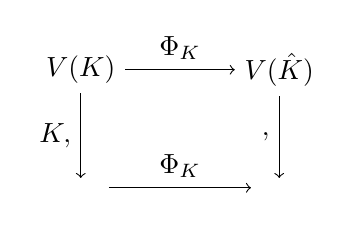
\begin{tikzpicture}
  \matrix[row sep=3em,column sep=4em,minimum width=2em]
  {
     \node(A) {$V(K)$}    ;& \node(B){$V(\hat K)$}; \\
     \node(C) {$\SpaceP$} ;& \node(D){$\RefP$}    ; \\};
     \draw[->] (A) -- (B) node[midway,above] {$\Phi_K$};
     \draw[->] (A) -- (C) node[midway,left] {$\Iop{K,\xV}$};
     \draw[->] (B) -- (D) node[midway,left] {$\Iop{\RefK,\xV}$};
     \draw[->] (C) -- (D) node[midway,above] {$\Phi_K$};
\end{tikzpicture}
\end{center}
which means that the interpolation operators and the transport of the elements commute: $\Iop{\RefK,\xV}\mathop{\circ}\Phi_K = \Phi_K\mathop{\circ} \Iop{K,\xV}$.

\begin{rmrk}
Note that in the literature the mapping between spaces is defined from $\xV(\CellK)$ to $\xV(\RefK)$, while the geometric mapping between cells is defined from $\RefK$ to $\CellK$. The affine-equivalence consists in the case $\Phi_K$ coinciding with $T_K^{-1}$. For Lagrange we defined $\Phi_K: \xCzero(K) \rightarrow \xCzero(\hat K)$ given by $v \mapsto v\mathop{\circ}T_K$.
In that case $\SpaceP = \Span\Fam{ \hat\varphi\circ T_K^{-1} }$ and the degrees of freedom are defined by $\Sigma = \Fam{\sigma_i : \sigma_i(v) = \hat\sigma_i(\Phi_K(v)) = \Phi_K(v)(\hat\xi_i) = v\mathop{\circ} T_K(\hat\xi_i)}$.
If $\xi_i = T_K(\hat\xi_i)$ then the definition is consistent.
\end{rmrk}



%\section{Non-conforming Finite Elements}

%-------------------------------------------------------------------------------
\section{Method}

\begin{lgrthm}[Finite Element Method]\label{alg:fem}

Solving a problem by a Finite Element Method is defined by the following procedure:
\begin{enumerate}
\item Choose a reference Finite Element $\RefFE$.
\item Construct an admissible mesh $\meshT$ such that any cell $\CellK \in \meshT$ is in bijection with the reference cell $\RefK$.
\item Define a mapping to transport the reference Finite Element defined on $\RefK$ onto any $\CellK \in \meshT$ to generate $\FE$.
\item Construct a basis for $\xVh$ by collecting all the shape functions of Finite Elements $\lbrace \FE \rbrace_{\CellK \in \meshT}$ sharing the same degree of freedom.

\end{enumerate}
\end{lgrthm}

%-------------------------------------------------------------------------------
\newpage

\section{Exercises}

\begin{tmaxrcs}{}{3.1}
Let us consider the Poisson problem posed on the domain $\dom = (0,1)$:
\begin{subequations}\label{pb:poisson_unit_fem}
\begin{equation}\label{pb:poisson_unit_eq_fem}
- u''(x) = f(x), \qquad\forany x\in\dom
\end{equation}
with $f\in \xLtwo(\dom)$, and satisfying the boundary condition on $\bound$
\begin{equation}\label{pb:poisson_unit_bc_fem}
u(x) = 0, \qquad\forany x\in\bound
\end{equation}
\end{subequations}
The domain $\bar\dom$ is discretized into a family of subintervals $[x_i, x_{i+1}]$, $i = 0,\cdots, N$, and Problem \ref{pb:poisson_unit_fem} is approximated by a linear Lagrange finite element method.
The approximation space is the space of continuous piecewise linear functions $V_h = \lbrace\varphi_i\rbrace_{0\leq i \leq N}$ with
\begin{equation}
\varphi_i(x) =
\left\lbrace
\begin{array}{l}
\displaystyle\frac{x - x_{i-1}}{x_i - x_{i-1}}\:,\quad x_{i-1}\leq x \leq x_{i},\:i \neq 0\\[2ex]
\displaystyle\frac{x_{i+1} - x}{x_{i+1} - x_{i}}\:,\quad x_{i}\leq x \leq x_{i+1},\:i \neq N\\[2ex]
0\quad otherwise
\end{array}
\right.
\end{equation}


\begin{tmatsks}
\item Find the weak formulation of Problem \ref{pb:poisson_unit_fem}.
\item Prove that $a(u - u_h, \varphi_i) = 0$, for $i = 1,\cdots,N-1$.
\item Prove that for any $v\in\xHone([0,1])\cap \xC^0([0,1])$, $i = 1,\cdots,N-1$:
\begin{equation}
a(v, \varphi_i) = \displaystyle\frac{1}{h}\bigl[- v(x_{i-1}) + 2v(x_i) - v(x_{i+1})\bigr]
\end{equation}
\end{tmatsks}

\medskip
Let us consider $f(x) = x^4$:
\begin{tmatsks}
\item Find the expression of the solution to Problem \ref{pb:poisson_unit_fem}.
\item Give the expression of the linear system obtained by the suggested method on a uniform grid, \ie $x_i = i h$, $i = 0,\cdots, N$.
\item Implement a program computing the discrete solution $u_h$ using the suggested method.
\item Plot the discrete solution $u_h$, the exact solution $u$, and the error $\snorm{u - u_h}$ with $N=8,16,32$.
\item Implement a function computing the $\xLtwo$ error-norm $\norm{u -u _h}_{\xLtwo(\dom)}$ and plot the value for different values of $N$.
\item Modify the program to handle non-uniform grids, given a list of node coordinates $\Fam{x_i}_{0\leq i\leq N}$.
\item Based on the error $\snorm{u -u _h}$ suggest a distribution of the nodes $\Fam{x_i}_{0\leq i\leq N}$, repeat the same study, then compare the error values.
\end{tmatsks}
\end{tmaxrcs}

